\documentclass{scrartcl}[12pt, halfparskip]
\usepackage[utf8x]{inputenc}
\usepackage[T1]{fontenc}
\usepackage[english]{babel}
\usepackage{amsmath, amssymb, amstext}
\usepackage{wrapfig}
\usepackage{float}
\usepackage{graphicx}
\usepackage{color}
\usepackage{booktabs}


\usepackage{caption}
\usepackage{subcaption}

\bibliographystyle{unsrt}

\setlength{\parindent}{0pt}

\newcommand{\todo}[1]{\textcolor{red}{TODO: #1}}
\newcommand{\bem}[1]{\textcolor{blue}{Bem.: #1}}


\title{Master Thesis}


\author{Jan Lammel}
\date{\today{}, Heidelberg}



\begin{document}

\begin{titlepage}
	\begin{center}
	
	\textsc{\large Ruprecht-Karls-Universit\"{a}t Heidelberg} \\[0.5cm]
	\textsc{\large Master Thesis}\\[1cm]
	
	\newcommand{\HRule}{\rule{\linewidth}{0.5mm}}
	\HRule \\[0.4cm]
	\huge \bfseries Ueberschrift
	\HRule 
	
	\vspace{11cm}
	
	\Large \textit{Jan Lammel }\\
	\Large \textit{Heidelberg, \today }\\ \vspace{0.5cm}
	\Large \textit{Supervisor:}
	
	\Large \textit{Prof. Dr. Dr. h. c. mult. Hans Georg Bock}\\
	\Large \textit{Dr. Andreas Sommer}
	
	\end{center}
\end{titlepage}

\newpage

\tableofcontents 
\newpage

 \pagenumbering{Roman} 
 

 \addsec{Abstract}
 bla bla bla
 
 
 \newpage

\addsec{Zusammenfassung}
blubb !

\newpage
\pagenumbering{arabic}
\section{Introduction}

\section{Physical Background}
\subsection{Heat equation}
As we are dealing with heat transport the central equation in this thesis is the


\subsection{Differential Scanning Calorimetry}
The measuring method of a heat flux into a sample over a certain temperature range is called Differential Scanning Calorimetry (DSC). 


\subsubsection{power compensated DSC}

\begin{wrapfigure}{r}[-2cm]{0.4\textwidth}
	\includegraphics[width=0.3\textwidth]{/home/argo/masterarbeit/thesis/images/DSC_principle.jpg}
	\caption{Working principle of power compensated DSC}
\end{wrapfigure}

In the case of a power compensated DSC (Fig. \ref{fig:DTA_principle}) there are 2 seperated chambers for a reference and the sample. Both have individual heaters and temperature sensors such that a feedback control system keep the temperature in both chambers on the same value. Since we know the electrical power for heating we can deduce on the heat flux due to energy conservation. \todo{Fuer was genau brauchen wir die Referenz?}




\subsubsection{heat flux DSC}

\begin{wrapfigure}{l}{0.4\textwidth}
	\includegraphics[width=0.3\textwidth]{/home/argo/masterarbeit/thesis/images/DTA_principle.jpg}
	\caption{Working principle DTA}
	\label{fig:DTA_principle}
\end{wrapfigure}

The heat flux DSC is based on differential thermal analysis (DTA, see Fig. \ref{fig:DTA_principle}). In DTA there is just one chamber in which both reference and sample are heated equally. Due to differences in the heat capacity of reference and sample a temperature difference dependent on their temperature will appear. This can be used to find typical temperatures of known substances to identify the sample's components.





\begin{figure}[H]
	\centering
	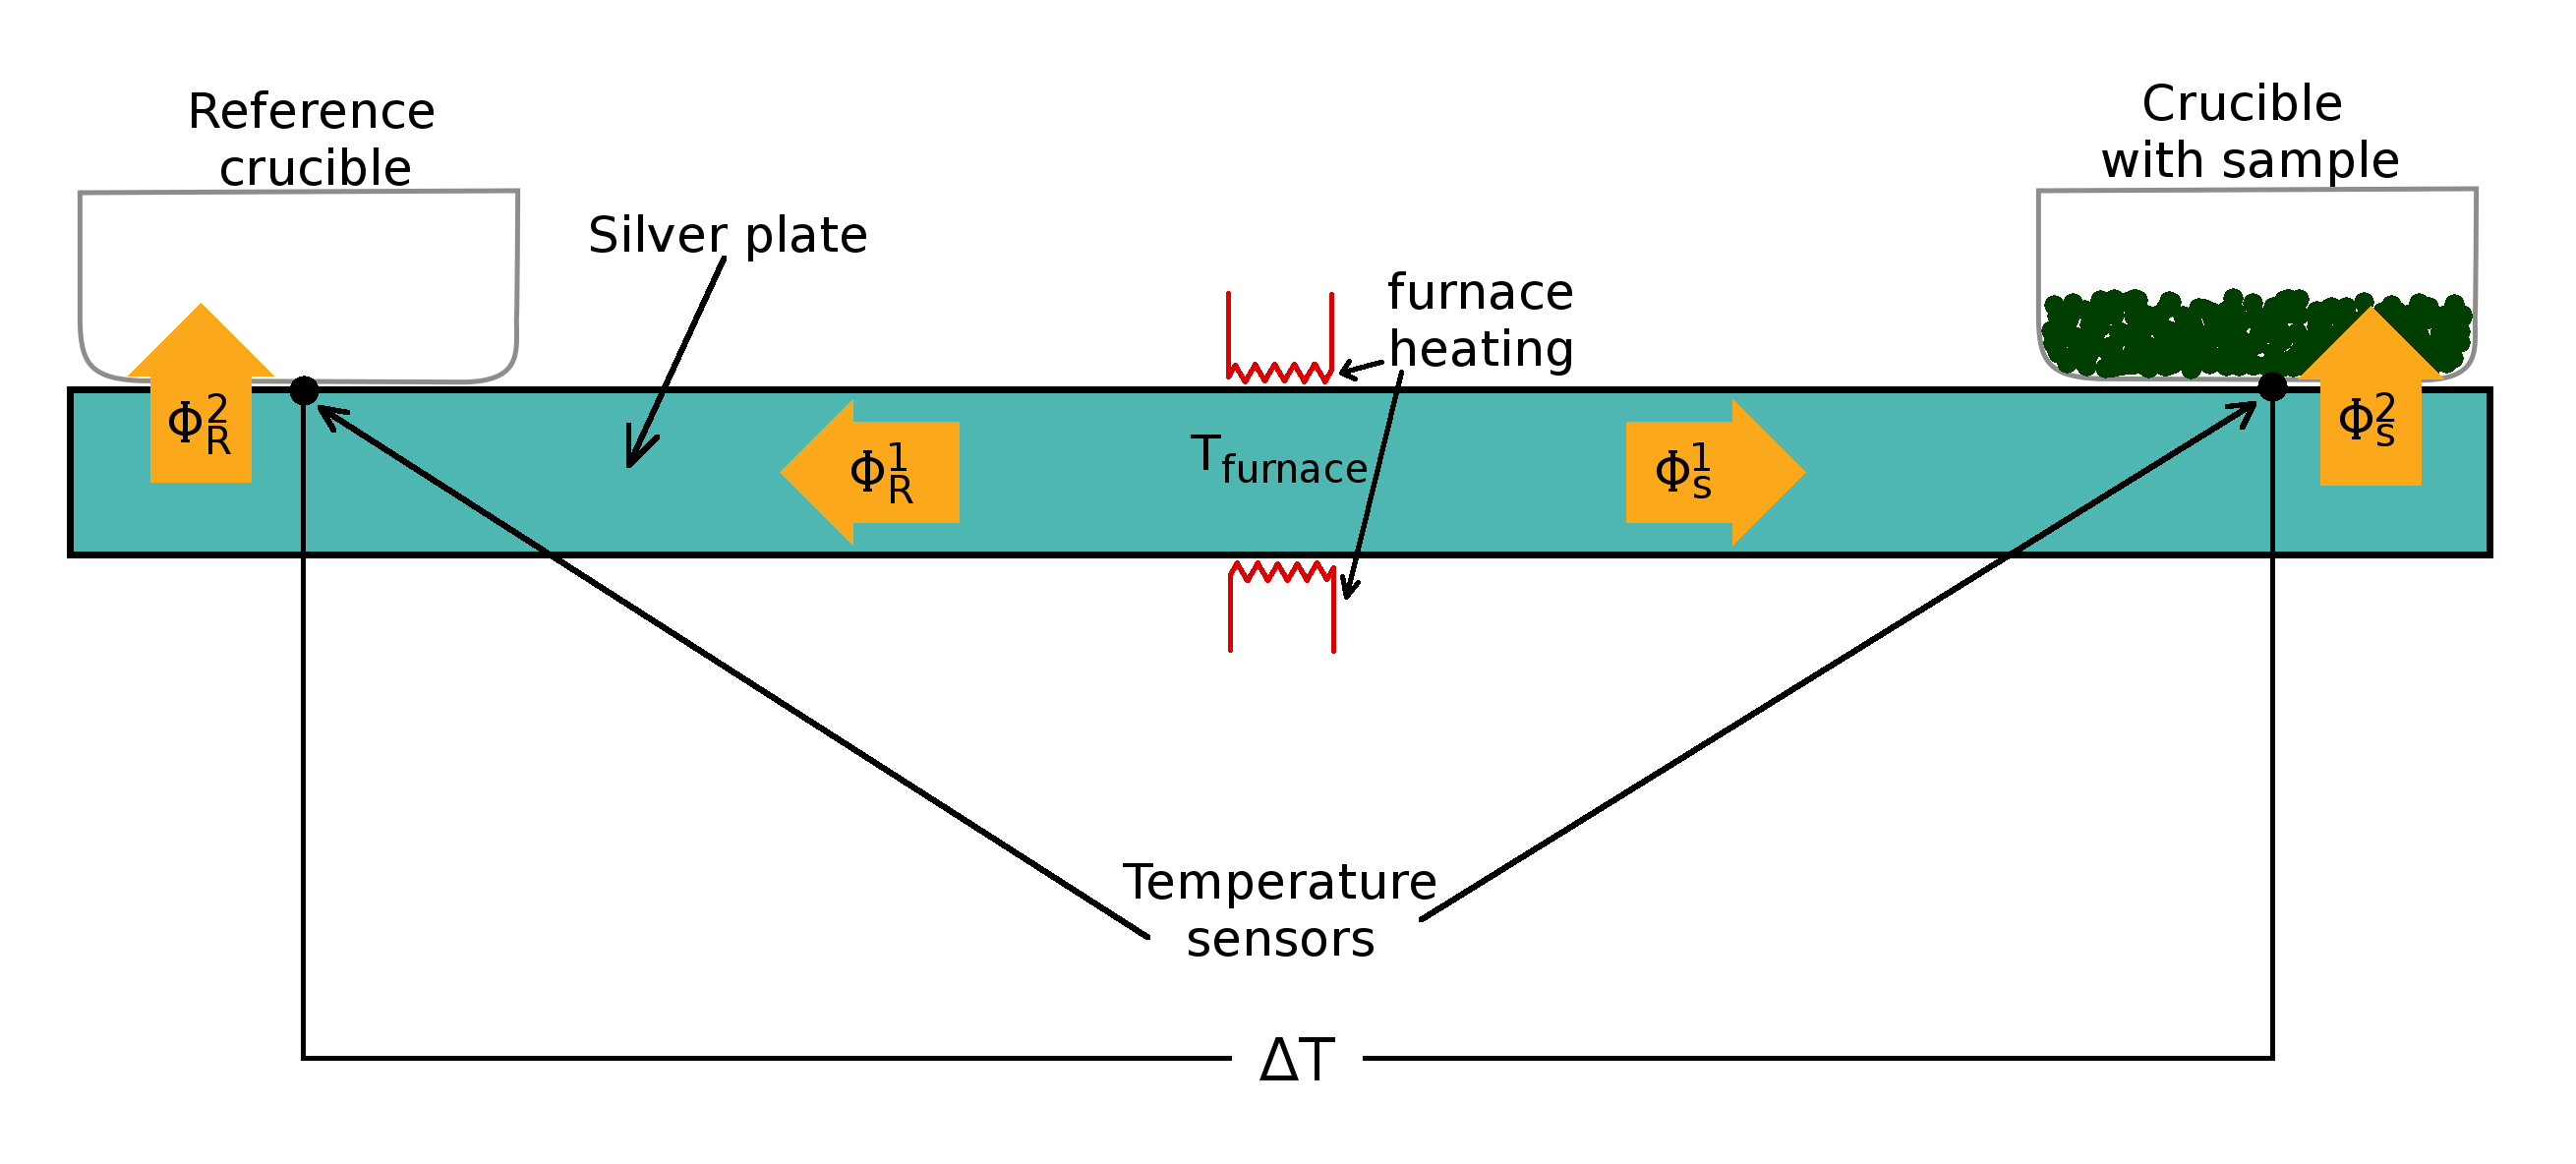
\includegraphics[width=1.\textwidth]{/home/argo/masterarbeit/thesis/images/dsc_funktionsprinzip.png}
	\caption{Principle experimental scheme of DSC which has been used for measurements.}
\end{figure}


\newpage
\section{Mathematical Background}
\subsection{Numerical integration of ODE systems}
\subsection{PDE discretization: Method of lines}

\subsection{Derivative generation}
In the context of continuous optimization we are dependent on derivative information in order to minimize some function. There are several possibilities to gain these derivatives. We will introduce here the concept of finite differences and automatic differentiation which were used in this thesis. Beside them the methods of symbolic- and complex step-differentiation exist and are explained in detail in \cite{diss_jan}.
\subsubsection{Finite Differences}
\bem{Wichtig weil wir am Anfang mit den NURBS noch finite Differenzen benutzt haben... ausserdem sind finite Differenzen auch fuer Linienmethode bei der PDE Diskretisierung notwendig.}\\

Derivatives generated by finite differences can be derived easily from Taylor-series expansion. Considering the function $f: \mathcal{R} \rightarrow \mathcal{R}^m$ the Taylor series looks as follows:
\begin{equation}
	f(x+h) = f(x) + h \cdot \frac{\partial f}{\partial x}(x) + \mathcal{O}(h^2)
\end{equation}

Reordering gives the one-sided derivative approximation

\begin{equation}
	\frac{\partial f}{\partial x}(x) = \frac{f(x+h) - f(x)}{h} + \mathcal{O}(h^2)
\end{equation}

Regarding the Taylor series up to order two in both directions of the domain of definition,

\begin{subequations}
\label{eq:finite_differences_taylor_exp}
\begin{align}
	f(x+h) = f(x) + h \cdot \frac{\partial f}{\partial x}(x) + \frac{h^2}{2} \cdot \frac{\partial^2 f}{\partial^2 x}(x) + \mathcal{O}(h^3) \label{eq:finite_differences_taylor_exp_+} \\
	f(x-h) = f(x) - h \cdot \frac{\partial f}{\partial x}(x) + \frac{h^2}{2} \cdot \frac{\partial^2 f}{\partial^2 x}(x) + \mathcal{O}(h^3)  \label{eq:finite_differences_taylor_exp_-}	
\end{align}
\end{subequations}


subtract both equations and reorder again we get

\begin{equation}
	\frac{\partial f}{\partial x}(x) = \frac{f(x+h) - f(x-h)}{2 h^2} + \mathcal{O}(h^3)
\end{equation}

which has a higher error order but at the expense of two function evaluations. \\

Second order derivatives can be gained analogously by adding \eqref{eq:finite_differences_taylor_exp_+} and \eqref{eq:finite_differences_taylor_exp_-}:

\begin{equation}
	\frac{\partial^2 f}{\partial^2 x}(x) = \frac{f(x-h) - 2 \cdot f(x) + f(x+h)}{h^2} + \mathcal{O}(h^3)
	\label{eq:finite_difference_2nd_der}
\end{equation}


\todo{Hier noch ne kleine Skizze einfuegen mit dem Diskretisierungsschema mit $\alpha$, und text vervollstaendigen} \\
In the spatial discretization of partial differential equations one often choose a finer grid for areas ...

\begin{subequations}
	\label{eq:finite_differences_taylor_exp_non-homogenous}
	\begin{align}
	f(x-h) = & f(x) - h \cdot \frac{\partial f}{\partial x}(x) + \frac{h^2}{2} \cdot \frac{\partial^2 f}{\partial^2 x}(x) + \mathcal{O}(h^3) \label{eq:finite_differences_taylor_exp_non-homogenous_1} \\
	f(x+\alpha h) = & f(x) - \alpha h \cdot \frac{\partial f}{\partial x}(x) + \frac{\alpha^2 h^2}{2} \cdot \frac{\partial^2 f}{\partial^2 x}(x) + \mathcal{O}(h^3)  \label{eq:finite_differences_taylor_exp_non-homogenous_2}
	\end{align}
\end{subequations}

Multiplying \eqref{eq:finite_differences_taylor_exp_non-homogenous_1} with $\alpha$ and adding \eqref{eq:finite_differences_taylor_exp_non-homogenous_2} gives

\begin{align}
	\alpha f(x-h) + f(x+\alpha h) = \alpha f(x) + \alpha \frac{h^2}{2} \frac{\partial^2 f}{\partial^2 x}(x) + f(x) + \frac{\alpha^2 h^2}{2} \frac{\partial^2 f}{\partial^2 x}(x) \\
	\Leftrightarrow (\alpha+1) \frac{\alpha h^2}{2} \frac{\partial^2 f}{\partial^2 x}(x) = \alpha f(x-h) - (\alpha+1) f(x) + f(x+\alpha h)
\end{align}

\begin{equation}
	\Leftrightarrow \frac{\partial^2 f}{\partial^2 x}(x) = \frac{1}{h^2} \left[ \frac{2}{1+\alpha} f(x-h) - \frac{2}{\alpha} f(x) + \frac{2}{\alpha (\alpha+1)} f(x+\alpha h) \right]
\end{equation}

Note that for a homogeneous grid ($\alpha=1$) this is obviously equal to \eqref{eq:finite_difference_2nd_der}. \\

For simplicity we restricted the function argument $x \in \mathcal{R}$. In the case $x \in \mathcal{R}^n$ the Jacobian is gained by performing directional derivatives. So e.g. for the one-sided first derivative $n+1$ function evaluations are necessary.

\todo{Vor-/Nachteile...} 



\subsubsection{Automatic Differentiation and Internal Numerical Differentiation}
The basic idea of Automatic Differentiation (AD) is to subdivide a function $f: \mathcal{R}^n \rightarrow \mathcal{R}^m$ into so called elementary functions $\varphi_i$ from which the derivative is known. 

The evaluation of these elementary functions give intermediate values $v_i = \varphi(v_j)_{j \prec i}$ where the dependency relation $\prec$ is defined as

\begin{equation}
	j \prec i \Leftrightarrow v_j \text{\textit{ is an argument of }} \varphi_i.
\end{equation}

By successively applying the chain rule one obtains the derivative of $f$.
One can distinguish the forward and reverse mode which will be explained in more detail now and exemplified by means of the example function

\begin{equation}
	F(x) = 
	\begin{bmatrix}
	\exp((1+x_1)^2) + x_3 \\
	x_2 \cdot \sin(1+x_1)
	\end{bmatrix}
\end{equation}

\todo{Graph mit den einzelnen Berechnungsverzweigungen noch einfuegen?}

\paragraph{Forward Mode}\mbox{}\\
In the forward mode the directional derivative $\dot{y}$ is computed for a given direction in the function arguments $\dot{x}$ at a evaluation point $x$:

\begin{equation}
	\dot{y} = \frac{\partial f}{\partial x}(x) \cdot \dot{x}
	\label{eq:AD_example}
\end{equation}

The algorithm called first order forward sweep is structured into three parts. First the auxiliary variables $v_{1-n},...,v_0$ and $\dot{v}_{1-n},...,\dot{v}_0$ are initialized with the evaluation point $x$ and the direction of the directional derivative $\dot{x}$. So if we want to get $\frac{\partial f}{\partial x_2}$ we would need to set $\dot{x} = \begin{bmatrix}
0 & 1 & 0 & \dots & 0
\end{bmatrix}^T$. One can see here that with one forward sweep we get one column of the Jacobian $ \frac{\partial f}{\partial x}$. 
After the initialization the actual forward sweep begins where the $k$ elemental functions of $f$ are evaluated and saved in the intermediate values $v_i$. Simultaneously their derivatives  $\dot{v}_i$ are computed using previously calculated intermediate values. E.g. for $v_2 = \varphi_2(v_0, v_1)$ it would hold $\dot{v}_2 = \frac{\partial \varphi_2}{\partial v_0} \dot{v_0} + \frac{\partial \varphi_2}{\partial v_1} \dot{v_1}$. \\
The last $m$ intermediate variables represent the solution vector. So finally this values and derivatives are extracted.


\todo{Q: Ist das hier eine totale Ableitung?}


\begin{table}[H]
\begin{tabular}{|c | l c l | l |} \hline
	 Initialization & $[v_{i-n}, \dot{v}_{i-n}]$ & $=$ & $[x_i, \dot{x}_i]$ & $i=1,...,n$ \\ \hline
	Intermediate steps & $[v_{i}, \dot{v}_{i}]$ & $=$ & $[\varphi_i(v_j)_{j \prec i}, \sum_{j \prec i} \frac{\partial \varphi_i}{\partial v_j}(v_j) \cdot \dot{v}_j]$ & $i=1,...,k$ \\ \hline
	Extract solution & $[y_{m-i}, \dot{y}_{m-i}]$ & $=$ & $[v_{k-i}, \dot{v}_{k-i}]$ & $i=m-1,...,0$ \\ \hline
\end{tabular}
\caption{First order forward sweep}
\label{tab:first_order_forward_sweep}
\end{table}

In order to illustrate this algorithm we will apply it onto the example function \eqref{eq:AD_example}:

\begin{table}[H]
\centering
\begin{tabular}{| c | l | l |} \hline
	Initialization & $v_{-2} = x_1$ & $\dot{v}_{-2} = \dot{x_1}$ \\
	& $v_{-1} = x_2$ & $\dot{v}_{-1} = \dot{x}_2$ \\
	& $v_{0} = x_3$ & $\dot{v_{0}} = \dot{x}_3$ \\ \hline
	Intermediate Steps & $v_1 = 1+v_{-2}$ & $\dot{v_1} = 1 \cdot \dot{v}_{-2}$ \\
	& $v_2 = v_{1}^2$ & $\dot{v_2} = 2 v_1 \cdot \dot{v}_{1}$ \\
    & $v_3 = \exp(v_{2})$ & $\dot{v_3} = \exp(v_2) \cdot \dot{v}_{2}$ \\
    & $v_4 = \sin(v_{1})$ & $\dot{v_4} = \cos(v_1) \cdot \dot{v}_{1}$ \\
	& $v_{5} = v_3 + v_0$ & $\dot{v_{5}} = 1 \cdot \dot{v}_3 + 1 \cdot \dot{v}_0$ \\
	& $v_{6} = v_{-1} + v_4$ & $\dot{v_{6}} = v_4 \cdot \dot{v}_{-1} + v_4 \cdot \dot{v}_{-1}$ \\ \hline
	Extract  solution & $y_1 = v_5$ & $\dot{y}_1 = \dot{v}_5$ \\
	& $y_2 = v_6$ & $\dot{y}_2 = \dot{v}_6$ \\ \hline
\end{tabular}
\caption{First order forward sweep applied on \eqref{eq:AD_example}.}
\end{table}




\paragraph{Adjoint Mode}\mbox{}\\
Beside the forward mode there is the adjoint mode where the adjoint directional derivative $\bar{x}^T$ is computed for a given adjoint direction $\bar{y}^T$ at the evaluation point $x$. 

\begin{equation}
	\bar{x}^T = \bar{y}^T \frac{\partial f}{\partial x}(x)
\end{equation}

The algorithm is shown in Table \ref{tab:first_order_adjoint_sweep}. In contrary to the forward mode we need here an additional set of adjoint intermediate variables $\bar{v}_i$. These contain the adjoint sensitivity information which are initialized to zero in the first step. \\
The following forward sweep is analog to the one shown in Table \ref{tab:first_order_forward_sweep}, however here we compute just the intermediate function evaluations without derivatives. We need these function values in the next part. \\
The actual adjoint directional derivatives are now computed in the reverse sweep which consists of three sub-steps. First of all the adjoint directions $\bar{y}$ is chosen. So for example, if we want the second row of the Jacobian $\frac{\partial f_2}{\partial x}$ we need to set $\bar{y} = \begin{bmatrix}
0 & 1 & 0 & \dots & 0
\end{bmatrix}^T$.
Next all contributions to the adjoint intermediate variables will be successively summed up by applying the adjoint equation $\bar{y}^T \dot{y} = \bar{y}^T J \dot{x} = \bar{x}^T \dot{x}$ in a reverse scheme (that is why we need the forward sweep and hence the intermediate value evaluations first). Finally we can extract the solution $\bar{x}$ which corresponds to a row in $\frac{\partial f}{\partial x}$.


\begin{table}[H]
\centering
\begin{tabular}{| c | l c l | l |} \hline
	Initialization & $\bar{v}_i$ & $=$ & $0$ & $i=1-n,...,k-m$ \\ \hline
	& $v_{i-n}$ & $=$ & $x_i$ & $i=1,...,n$ \\
	Forward Sweep & $v_{i}$ & $=$ & $\varphi_i(v_j)_{j \prec i}$ & $i=1,...,k$ \\
	& $y_{m-i}$ & $=$ & $v_{k-i}$ & $i=m-1,...,0$ \\ \hline
	& $\bar{v}_{k-i}$ & $=$ & $\bar{y}_{m-i}$ & $i=0,...,m-1$ \\
	Reverse Sweep & $\bar{v}_j$ & $+ \hspace{-0.1cm} =$ & $\bar{v}_i \frac{\partial \varphi_i}{\partial v_j}(v_j) \quad \forall \ j \prec i$ & $i=k,...,1$ \\
	& $\bar{x}_i$ & $=$ & $\bar{v}_{i-n}$ & $i=n,...,1$ \\ \hline
\end{tabular}
\caption{First order adjoint sweep}
\label{tab:first_order_adjoint_sweep}
\end{table}

Again we apply this algorithm on the exemplary function \eqref{eq:AD_example}:

\begin{table}[H]
\centering
\begin{tabular}{| c | l | l |} \hline
	Initializiation & $\bar{v}_{-2}=\dots=\bar{v}_4=0$ & \\ \hline
	& \textbf{Forward Sweep} & \textbf{Reverse Sweep} \\ \hline
	Initialization & $v_{-2}=x_1$ & $\bar{v}_6=\bar{y}_2$ \\
	& $v_{-1}=x_2$ & $\bar{v}_5=\bar{y}_1$ \\
	& $v_{0}=x_3$ &  \\	\hline
	Sweep & $v_1=1+v_{-2}$ & $\bar{v}_{-1} +\hspace{-0.1cm}= \bar{v}_6 \cdot v_4$ \\
	& $v_2=v_{1}^2$ & $\bar{v}_{4} +\hspace{-0.1cm}= \bar{v}_6 \cdot v_{-1} $ \\
	& $v_3=\exp(v_2)$ & $\bar{v}_{3} +\hspace{-0.1cm}= \bar{v}_5 \cdot 1 $ \\
	& $v_4= \sin(v_1)$ & $\bar{v}_{0} +\hspace{-0.1cm}= \bar{v}_5 \cdot 1 $ \\
	& $v_5=v_{3} + v_0$ & $\bar{v}_{1} +\hspace{-0.1cm}= \bar{v}_4 \cdot \cos(v_1) $ \\
	& $v_6=v_{-1} \cdot v_4$ & $\bar{v}_{2} +\hspace{-0.1cm}= \bar{v}_3 \cdot \exp(v_2) $ \\
	& & $\bar{v_1} +\hspace{-0.1cm}= \bar{v}_2 \cdot 2 v_1$ \\
	& & $\bar{v_{-2}} +\hspace{-0.1cm}= \bar{v}_1 \cdot 1$	\\ \hline
	Extract solution & $y_1 = v_5$ & $\bar{x}_3 = \bar{v}_0$ \\
	& $y_2 = v_6$ & $\bar{x}_2 = \bar{v}_{-1}$ \\
	& & $\bar{x}_1 = \bar{v}_{-2}$	\\ \hline
\end{tabular}
\caption{First order adjoint sweep applied on \eqref{eq:AD_example}}
\end{table} 


Until now the fundamental principles of AD have been explained, i.e. just the first order derivative in forward and adjoint mode. Higher derivatives of arbitrary order can be obtained by using the method of Taylor coefficient propagation which is based on the propagation of a Taylor polynomial through a function evaluation. The higher derivatives can then be extracted by scaling of the polynomial coefficients. \\

In this thesis we are actually interested in the sensitivities $\frac{\partial y}{\partial p}$ of an differential equation $\dot{y}=f(t,y;p)$ with respect to parameters $p$. The application of AD on differential equations is called Internal Numerical Differentiation (IND). The principle is based on the fact that solving numerically a differential equation consists of many elemental operations from which the derivatives are known. So it is straight forward to apply the chain rule on all these elemental operations in order to get the derivative $\frac{\partial y}{\partial p}$ just as explained above. \\
A detailed explanation on taylor coefficient propagation for higher derivatives and IND can be found in \cite{diss_jan}. \todo{Reicht das... mehr?}


\paragraph{}\mbox{}\\



\subsection{Optimization Task: Parameter Estimation}


\newpage
\section{Simulation of DSC measuring process and parameter estimation of specific heat capacity $c_p$}
\subsection{Mathematical model}

\begin{figure}[H]
	\centering
	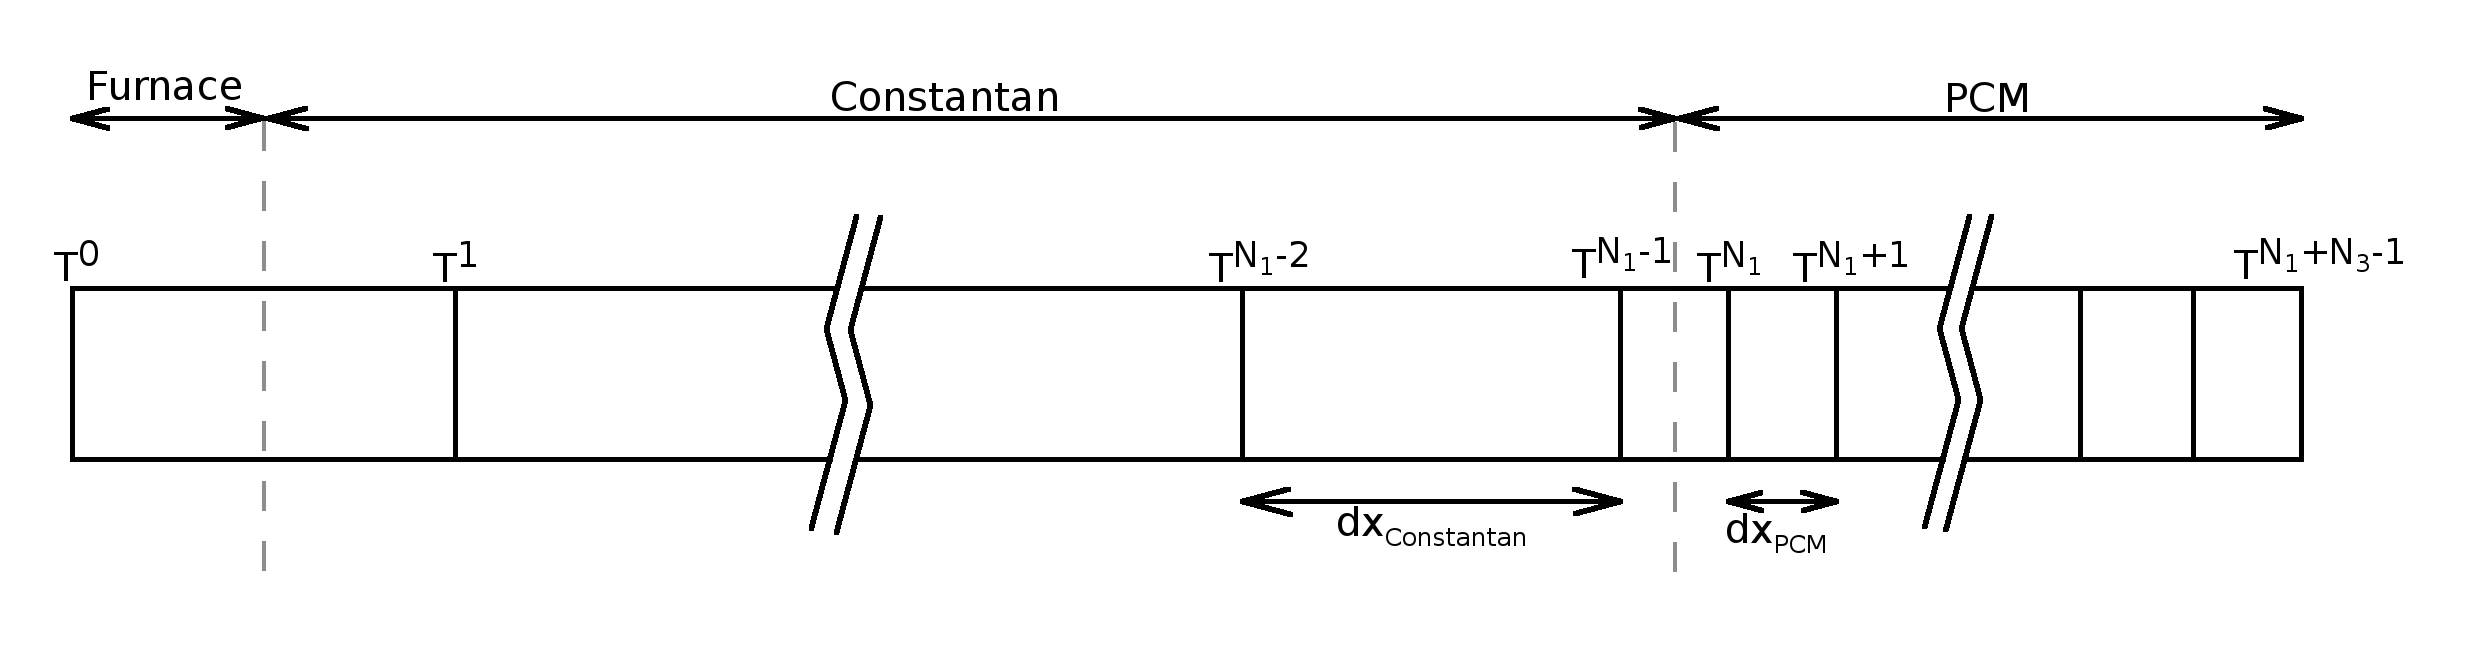
\includegraphics[width=1.\textwidth]{/home/argo/masterarbeit/thesis/images/discretization_grid.png}
	\caption{blubb}
\end{figure}



\subsection{Analytical solution of reference side}
\subsection{Parametrizations of $c_p$}
\subsection{Influence of spatial discretization grid}




\begin{thebibliography}{9}

\bibitem{diss_jan}
	 Adjoint-based algorithms and numerical methods for sensitivity generation and optimization of large scale dynamic systems, 
	 Jan Albersmeyer, 2010,
	 http://www.ub.uni-heidelberg.de/archiv/11651
\bibitem{DSC_buch}
	Differential Scanning Calorimetry of Polymers: physics, chemistry, analysis, technology,
	Vladimir A. Bershtein, Victor M. Egorov,
	1994

  
\end{thebibliography}

\end{document}